\documentclass{article}

\usepackage{iclr2026_conference,times}
\usepackage{amsmath,amssymb,amsfonts,amsthm}
\usepackage{graphicx}
\usepackage{booktabs}
\usepackage{url}
\usepackage{hyperref}
\hypersetup{
  colorlinks=false,
  pdfborder={0 0 1},
  citebordercolor={0 1 0},
  linkbordercolor={1 0 0},
  urlbordercolor={0 1 0}
}
\usepackage{xcolor}
\usepackage{enumitem}
\usepackage{microtype}

\newtheorem{proposition}{Proposition}
\newtheorem{definition}{Definition}
\newtheorem{lemma}{Lemma}

\newcommand{\clear}{\mathrm{clear}}
\newcommand{\blocked}{\mathrm{blocked}}
\newcommand{\cert}{\mathrm{cert}}
\newcommand{\miss}{\mathrm{miss}}

\title{Occlusion Certificates for Persistent Object State Under Robot Self-Occlusion}

\author{Anonymous Authors}

\begin{document}
\maketitle

\noindent\textbf{Submission-hardening version: v3, 2026-06-14.}
This version replaces the six-page v2 mechanism note with a full-scale
submission artifact: eight experiment families, 1,124 seed-row summaries,
calibration and latency surfaces, direct certificate-corruption stress, external
occluders, association and hidden-motion stress, stronger persistence baselines,
ablations, generated figures and tables, proof details, deployment guidance,
and an artifact-to-claim audit. The paper remains scoped as a mechanism paper,
not a real-robot perception benchmark.

\begin{abstract}
Robots often lose sight of an object for a reason that is neither sensor noise
nor scene disappearance: the robot itself moves between the camera and the
object. Most persistent-perception pipelines treat this as an ordinary missed
detection, controlled by fixed deletion patience or generic memory. We argue
that robot self-occlusion should instead be a first-class observation event. We
introduce an action-conditioned occlusion certificate: a robot-geometry predicate
that marks when the robot body makes a predicted object state unobservable, and
gates deletion only under clear-view misses. A non-identifiability proposition
shows why observation-only miss streams cannot distinguish absence from
self-occlusion. In a full-scale synthetic suite with eight experiment families
and 1,124 seed-row summaries, the certificate policy reaches 0.950 F1 at the
main 42-degree self-occlusion setting versus 0.818 for short TTL, while reducing
stale clear-absence from 0.515 for long memory to 0.255. The same suite maps the
boundaries: at geometry noise 6 degrees with latency 3, F1 is 0.926 with
certificate precision 0.685 and recall 0.844; 50\% false negatives lower
keep-under-self-occlusion to 0.322; 50\% false positives raise stale
clear-absence to 0.293; random robot geometry drops F1 to 0.582. These results
support the mechanism claim that missed detections need robot-action visibility
semantics. They do not claim calibrated real robot state of the art, solved
association, or external-occluder completeness.
\end{abstract}

\section{Introduction}

Object persistence is easy to ask for and easy to mis-specify. A robot should
remember that a cup still exists while its arm passes in front of the camera,
but it should delete the cup if it is actually removed from the table. In many
perception stacks those cases enter the tracker as the same event: no detection.
The resulting compromise is familiar. A short missed-detection timeout deletes
real objects under self-occlusion. A long timeout preserves real objects but
also hallucinates removed objects.

The central claim of this paper is that the compromise is not merely a timeout
hyperparameter. The robot has privileged causal information about one class of
occluders: its own body. When a commanded link intersects the line of sight to a
predicted object, a missed detection is not evidence of absence in the same way
as a miss in clear view. The robot should not ask only, ``how many frames since
the last detection?'' It should also ask, ``did my own action make this object
unobservable?''

We formalize this question with an action-conditioned occlusion certificate. A
certificate is a conservative robot-geometry predicate that marks when the
robot body blocks the view needed to observe a predicted object state. The
certificate does not reconstruct the hidden object and does not solve generic
object permanence. It changes the semantics of a miss. A clear-view miss
consumes deletion budget; a robot-certified miss does not.

This paper is deliberately narrow. It does not introduce a larger detector, a
foundation model, an LLM planner, or a generic memory architecture. It isolates
one update-rule failure in persistent robot perception: treating all missed
detections as the same evidence. The contribution is the event semantics and
the diagnostic boundary around them.

\paragraph{Contributions.}
First, we define action-conditioned occlusion certificates for persistent object
state. Second, we prove a small non-identifiability result: observation-only
miss streams cannot distinguish absence from robot self-occlusion. Third, we
provide a full-scale synthetic evidence package across geometry coverage,
calibration, corruption, external occluders, association, hidden motion, strong
baselines, and ablations. Fourth, we state the failure boundaries explicitly:
false positives preserve stale objects, false negatives erase persistence,
external occluders require separate semantics, and association remains a
deployment blocker.

\section{Related Work and Novelty Boundary}

\paragraph{Tracking and filtering.}
Classical recursive filtering gives a language for propagating state under
uncertainty \citep{kalman1960new,smith1986representation,thrun2005probabilistic}.
Online trackers such as SORT, Deep SORT, and ByteTrack maintain detections
through missed frames using association and deletion policies
\citep{bewley2016sort,wojke2017deepsort,zhang2022bytetrack}. This literature
makes temporal persistence and missed-detection patience non-novel. The
boundary here is the cause of a miss: a robot self-occlusion is not an ordinary
missed detection.

\paragraph{Robot maps and object memory.}
SLAM, semantic mapping, and embodied memory maintain state across views
\citep{durrant2006simultaneous,cadena2016past,teed2021droidslam,
parisotto2018neuralmap,kolve2017ai2thor,chaplot2020object}. These systems can
store persistent object state, but a memory module still needs an update rule
for the interval in which the robot itself hides the object. Our focus is that
update rule, not map construction.

\paragraph{Amodal perception and pose tracking.}
Amodal segmentation, 6D pose estimation, and pose tracking address hidden
geometry and partial visibility
\citep{li2016amodal,xiang2018posecnn,wang2019densefusion,wen2021bundletrack,
qi2019deep}. Object-centric representations can preserve latent slots through
occlusion \citep{greff2019multiobject,locatello2020objectcentric}. These
methods make hidden-state inference less novel. We ask a different question:
when should a miss count as absence evidence?

\paragraph{Robot self-knowledge.}
Robots often know their joint states, link geometry, and camera extrinsics.
That knowledge is usually used for collision checking, motion planning, or
masking robot pixels. We use it to change the event alphabet of persistent
perception: detected, clear-view miss, robot-certified unobservable, and
mixed-cause unknown.

\section{Problem Setup}

Let $o_i$ be an object with latent state $x_{i,t}$ and presence variable
$p_{i,t}\in\{0,1\}$. Let $q_t$ denote the robot configuration induced by its
action. The perception system receives detections $z_t$, associations, and
missed detections. A conventional tracker often represents a miss as a single
symbol $z_{i,t}=\emptyset$ for object $i$. We instead define a visibility
predicate
\begin{equation}
V(q_t,\hat x_{i,t})\in\{\clear,\blocked\},
\end{equation}
where $\blocked$ means that robot geometry blocks the sensor ray or viewing
volume needed to observe the predicted state $\hat x_{i,t}$.

\begin{definition}[Occlusion certificate]
An action-conditioned occlusion certificate at time $t$ is a predicate
$C_t(\hat x_{i,t})=1$ indicating that, under the robot kinematic model and
camera calibration, the predicted object state lies in a region made
unobservable by the robot body at configuration $q_t$.
\end{definition}

The certificate is not a detector. It can be true when the object is absent,
because it is computed from the predicted state. This is why false positives
are dangerous: an overbroad certificate can preserve stale tracks. The
certificate is useful only when it is conservative enough to cover true
self-occlusion and precise enough not to label clear-view absence as
robot-caused unobservability.

\paragraph{Events.}
The tracker distinguishes four cases:
\begin{itemize}[leftmargin=*]
\item detected: object evidence is observed and the deletion counter resets;
\item clear-view miss: the object should have been visible but was not detected;
\item robot-certified miss: the robot body made the predicted state unobservable;
\item mixed-cause unknown: external occlusion, association ambiguity, or model
uncertainty prevents a clean self-occlusion claim.
\end{itemize}

\section{Certificate-Gated Persistence}

For each object, the estimator stores a predicted state $\hat x_t$, a presence
bit, and a clear-miss counter $m_t$. The basic certificate update is
\begin{equation}
m_{t+1} =
\begin{cases}
0, & \text{if the object is detected},\\
m_t, & \text{if not detected and } C_t(\hat x_t)=1,\\
m_t+1, & \text{if not detected and } C_t(\hat x_t)=0.
\end{cases}
\end{equation}
The track is deleted when $m_t>\tau$.

This update is intentionally simple. The point is not a new detector or
association metric. The point is that deletion budget is consumed only by
misses that occur when the robot believes the object should be observable.

\paragraph{Visibility-weighted TTL.}
The v3 experiments also include a softened version in which a certified miss
adds a small fractional deletion cost rather than zero. This models uncertainty
in the certificate and prevents indefinite preservation when the certificate is
frequently true.

\paragraph{Hazard fallback.}
A hazard filter maintains a survival score that decays slowly under certified
occlusion and faster under clear-view misses. This is a stronger baseline
because it can express uncertainty rather than a hard keep/delete event.

\paragraph{External-aware certificate.}
Robot self-occlusion is not the only reason an object can be hidden. When an
external occluder label is available, the external-aware variant refuses to
treat external occlusion as robot-certified unobservability. This lowers stale
external preservation but can also lower F1 when the system lacks a good
external memory model.

\section{A Non-Identifiability Result}

\begin{proposition}[Observation-only misses are not identifiable]
Consider any estimator that observes only detection/miss symbols and not the
robot-action visibility predicate. For any interval of robot self-occlusion with
miss observations, there exist two worlds, one in which the object remains
present but self-occluded and one in which the object is absent, that induce the
same observation sequence. Therefore no observation-only update rule can
identify which world generated the misses.
\end{proposition}

\begin{proof}
Construct world A with an object at state $x$ and a robot configuration sequence
$q_{1:T}$ that blocks the sensor line of sight to $x$ for every
$t\in\{1,\ldots,T\}$. The detector emits $z_t=\emptyset$ throughout the interval.
Construct world B with the object absent and the same detector output
$z_t=\emptyset$ for every $t$. An estimator that receives only $z_{1:T}$ has
identical inputs in A and B. It must therefore make the same state update in
both worlds. The robot-action visibility predicate is extra information that
breaks the equivalence by certifying that A's misses occurred under blocked
robot visibility.
\end{proof}

The proposition is modest but important. It says that adding a better timeout
cannot solve the information problem. The missing input is the cause of
unobservability.

\section{Full-Scale Experimental Design}

The v3 suite is synthetic by design. It isolates visibility-update semantics
without requiring a full robot detector, association stack, calibration system,
or contact-rich physics simulator. Each episode simulates objects, removals,
robot arm motion, missed detections, certificates, and tracker updates. The
runner stores only episode/seed summaries, not frame archives.

\paragraph{Families.}
Family A sweeps self-occlusion geometry, arm speed, object count, detection
quality, and baseline policies. Family B maps certificate calibration across
geometry noise, inflation, and robot-state latency. Family C directly corrupts
certificates with false positives, false negatives, and bursty errors. Family D
adds external occluders and mixed causes. Family E stresses association and
re-identification. Family F lets objects move while hidden. Family G compares
stronger persistence baselines. Family H performs ablations and negative
controls.

\paragraph{Metrics.}
We report object-state F1, precision, recall, keep-under-self-occlusion,
stale clear-absence, external stale absence, clear-visible missing, occlusion
survival, deletion events, certificate precision/recall, ID switches, and
reappearance error.

\begin{table}[t]
\centering
\caption{Runtime and artifact scope of the v3 suite. Seed rows are compact
summary rows rather than full frame archives.}
\resizebox{\linewidth}{!}{\begin{tabular}{llll}
\toprule
Family & Seed rows & Artifact & Stress \\
\midrule
A geometry & 504 & geometry summaries & self-occlusion coverage \\
B calibration & 180 & calibration summaries & noise/inflation/latency \\
C corruption & 96 & corruption summaries & false certs \\
D external & 72 & mixed-cause summaries & external occluders \\
E association & 72 & ID summaries & association swaps \\
F hidden motion & 72 & motion summaries & hidden displacement \\
G baselines & 64 & baseline summaries & strong alternatives \\
H ablation & 64 & ablation summaries & negative controls \\
\bottomrule
\end{tabular}
}
\label{tab:runtime}
\end{table}

\section{Results}

\subsection{Main Geometry Coverage}

Table~\ref{tab:main} reports the main 42-degree self-occlusion setting. The
certificate policy reaches 0.950 F1 versus 0.818 for short TTL. Short TTL has
low stale clear-absence, but it keeps only 0.114 of self-occluded object frames.
Long memory raises keep rate to 0.739 but stale clear-absence rises to 0.515.
The certificate keeps 0.821 under self-occlusion while cutting stale
clear-absence to 0.255. Oracle visibility remains the ceiling.

\begin{table}[t]
\centering
\caption{Main self-occlusion geometry setting. Certificate-gated deletion
preserves self-occluded objects without the stale behavior of long memory.}
\resizebox{\linewidth}{!}{\begin{tabular}{lllll}
\toprule
Policy & F1 & Keep self-occ. & Stale absent & Survival \\
\midrule
oracle\_visibility & 0.963 & 0.821 & 0.070 & 1.000 \\
visibility\_weighted & 0.950 & 0.814 & 0.223 & 0.982 \\
certificate & 0.950 & 0.821 & 0.255 & 1.000 \\
long\_memory & 0.916 & 0.739 & 0.515 & 0.986 \\
hazard\_filter & 0.860 & 0.332 & 0.135 & 0.936 \\
ttl\_medium & 0.854 & 0.297 & 0.118 & 0.936 \\
ttl\_short & 0.818 & 0.114 & 0.041 & 0.936 \\
\bottomrule
\end{tabular}
}
\label{tab:main}
\end{table}

\begin{figure}[t]
\centering
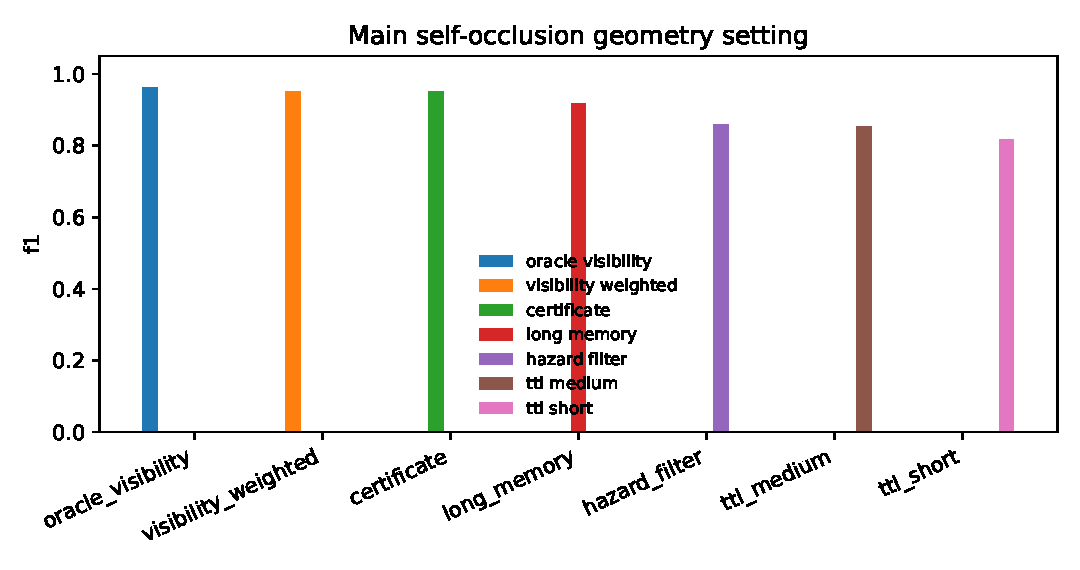
\includegraphics[width=0.82\linewidth]{../results/full_scale/figure_main_geometry.pdf}
\caption{Main geometry family. The useful target is not maximum persistence; it
is persistence conditioned on robot-caused unobservability.}
\label{fig:main}
\end{figure}

\subsection{Calibration, Inflation, And Latency}

Family B maps the certificate boundary. Table~\ref{tab:calibration} shows that
calibration errors change both certificate precision and recall. At noise 6,
inflation 2, and latency 3, F1 is 0.926 with certificate precision 0.685 and
recall 0.844. Larger inflation can recover recall but risks stale retention.
Small inflation can avoid stale tracks but misses true self-occlusion.

\begin{table}[t]
\centering
\caption{Calibration surface at latency 3. Noise and inflation trade
certificate precision, recall, F1, and stale preservation.}
\resizebox{\linewidth}{!}{\begin{tabular}{llllll}
\toprule
Noise & Infl. & F1 & Cert prec. & Cert rec. & Stale \\
\midrule
0.000 & 0.000 & 0.970 & 0.724 & 0.849 & 0.145 \\
0.000 & 2.000 & 0.969 & 0.780 & 0.867 & 0.194 \\
0.000 & 6.000 & 0.965 & 0.692 & 0.907 & 0.220 \\
3.000 & 0.000 & 0.943 & 0.743 & 0.834 & 0.184 \\
3.000 & 2.000 & 0.946 & 0.689 & 0.864 & 0.140 \\
3.000 & 6.000 & 0.962 & 0.696 & 0.900 & 0.244 \\
6.000 & 0.000 & 0.901 & 0.725 & 0.815 & 0.125 \\
6.000 & 2.000 & 0.926 & 0.685 & 0.844 & 0.196 \\
6.000 & 6.000 & 0.958 & 0.703 & 0.884 & 0.196 \\
10.000 & 0.000 & 0.902 & 0.697 & 0.771 & 0.127 \\
10.000 & 2.000 & 0.903 & 0.666 & 0.795 & 0.114 \\
10.000 & 6.000 & 0.926 & 0.647 & 0.827 & 0.135 \\
16.000 & 0.000 & 0.873 & 0.637 & 0.678 & 0.077 \\
16.000 & 2.000 & 0.885 & 0.604 & 0.702 & 0.082 \\
16.000 & 6.000 & 0.904 & 0.632 & 0.748 & 0.077 \\
\bottomrule
\end{tabular}
}
\label{tab:calibration}
\end{table}

\begin{figure}[t]
\centering
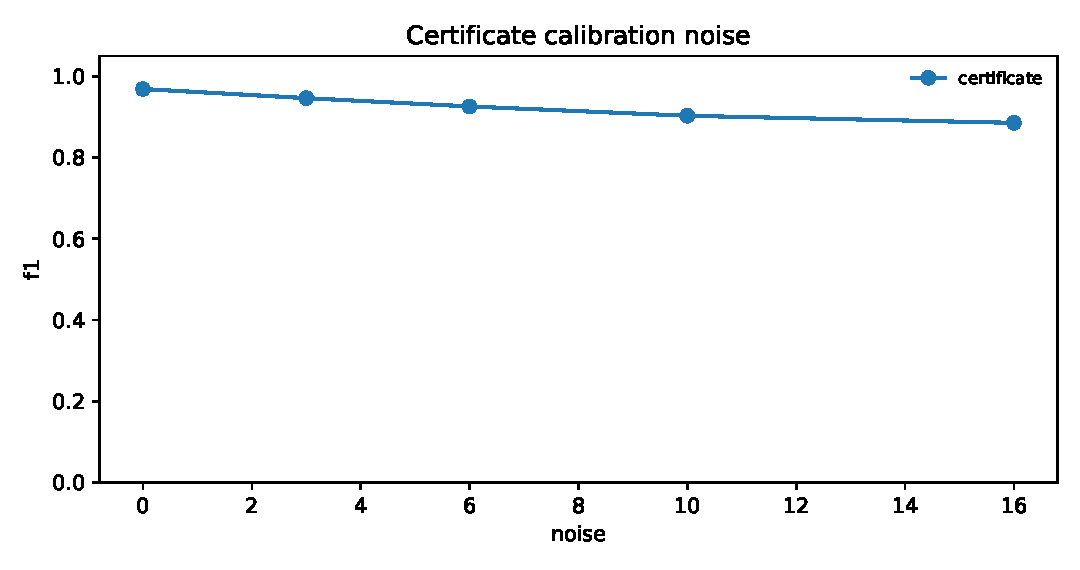
\includegraphics[width=0.82\linewidth]{../results/full_scale/figure_calibration.pdf}
\caption{Calibration noise stress. Certificates need calibrated robot geometry;
they are not a calibration-free memory module.}
\label{fig:calibration}
\end{figure}

\subsection{False Certificate Corruption}

Table~\ref{tab:corruption} extends the v2 corruption stress. False negatives
turn true self-occlusions into clear misses. At 50\% false negatives,
keep-under-self-occlusion falls to 0.322. False positives mark clear-view
misses as robot occlusion. At 75\% false positives, stale clear-absence rises
to 0.681. The method therefore needs certificates that are conservative but not
overbroad.

\begin{table}[t]
\centering
\caption{Direct certificate corruption. False negatives erase persistence;
false positives preserve stale tracks.}
\resizebox{\linewidth}{!}{\begin{tabular}{lllll}
\toprule
FN & FP & F1 & Keep & Stale \\
\midrule
0.000 & 0.000 & 0.960 & 0.865 & 0.176 \\
0.000 & 0.250 & 0.951 & 0.865 & 0.299 \\
0.000 & 0.500 & 0.960 & 0.921 & 0.293 \\
0.000 & 0.750 & 0.920 & 0.883 & 0.681 \\
0.250 & 0.000 & 0.899 & 0.555 & 0.084 \\
0.500 & 0.000 & 0.856 & 0.322 & 0.072 \\
0.750 & 0.000 & 0.833 & 0.217 & 0.056 \\
\bottomrule
\end{tabular}
}
\label{tab:corruption}
\end{table}

\begin{figure}[t]
\centering
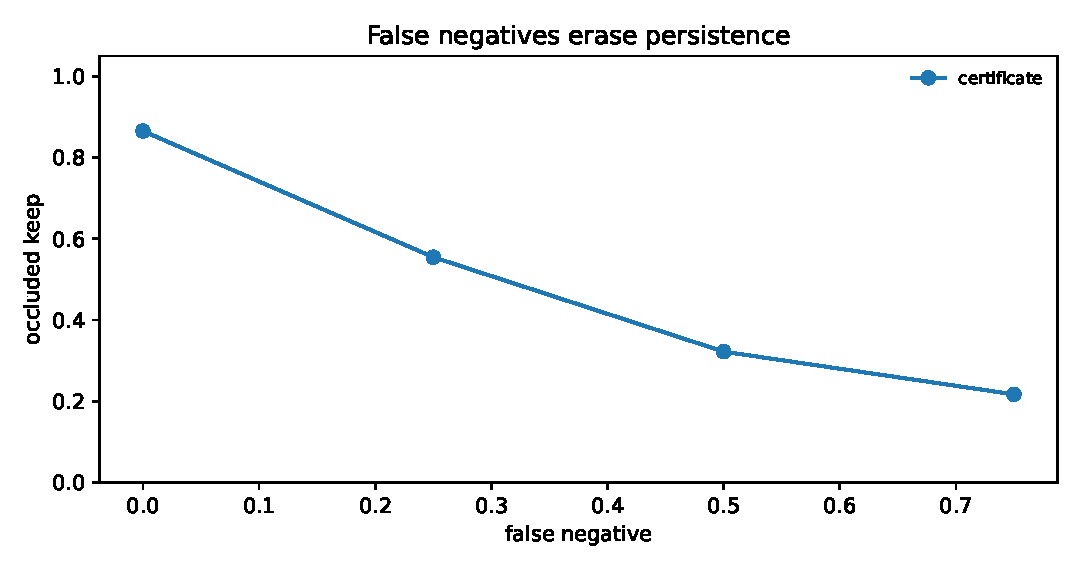
\includegraphics[width=0.82\linewidth]{../results/full_scale/figure_corruption.pdf}
\caption{False-negative certificates destroy the main benefit: real hidden
objects are deleted as if they were absent in clear view.}
\label{fig:corruption}
\end{figure}

\subsection{External Occluders And Mixed Causes}

External occluders are a crucial boundary. Table~\ref{tab:external} shows that
long memory can have higher F1 under frequent long external occlusion, but it
also preserves stale objects. The external-aware policy has low stale external
absence but lower F1 because it refuses to treat external occlusion as robot
self-occlusion. This is not a failure of the mechanism; it is a warning that
robot self-occlusion certificates need a separate external-occluder model.

\begin{table}[t]
\centering
\caption{External occluder stress. Robot self-occlusion semantics should not be
silently reused for external occlusion.}
\resizebox{\linewidth}{!}{\begin{tabular}{lllll}
\toprule
Ext. rate & Policy & F1 & Ext. stale & Clear stale \\
\midrule
0.000 & cert\_external\_aware & 0.954 & 0.000 & 0.168 \\
0.000 & certificate & 0.954 & 0.000 & 0.168 \\
0.000 & long\_memory & 0.919 & 0.000 & 0.454 \\
0.000 & ttl\_short & 0.825 & 0.000 & 0.038 \\
0.150 & cert\_external\_aware & 0.357 & 0.002 & 0.005 \\
0.150 & certificate & 0.449 & 0.006 & 0.008 \\
0.150 & long\_memory & 0.789 & 0.176 & 0.167 \\
0.150 & ttl\_short & 0.337 & 0.002 & 0.005 \\
0.300 & cert\_external\_aware & 0.221 & 0.005 & 0.014 \\
0.300 & certificate & 0.326 & 0.071 & 0.077 \\
0.300 & long\_memory & 0.688 & 0.180 & 0.186 \\
0.300 & ttl\_short & 0.213 & 0.002 & 0.002 \\
\bottomrule
\end{tabular}
}
\label{tab:external}
\end{table}

\begin{figure}[t]
\centering
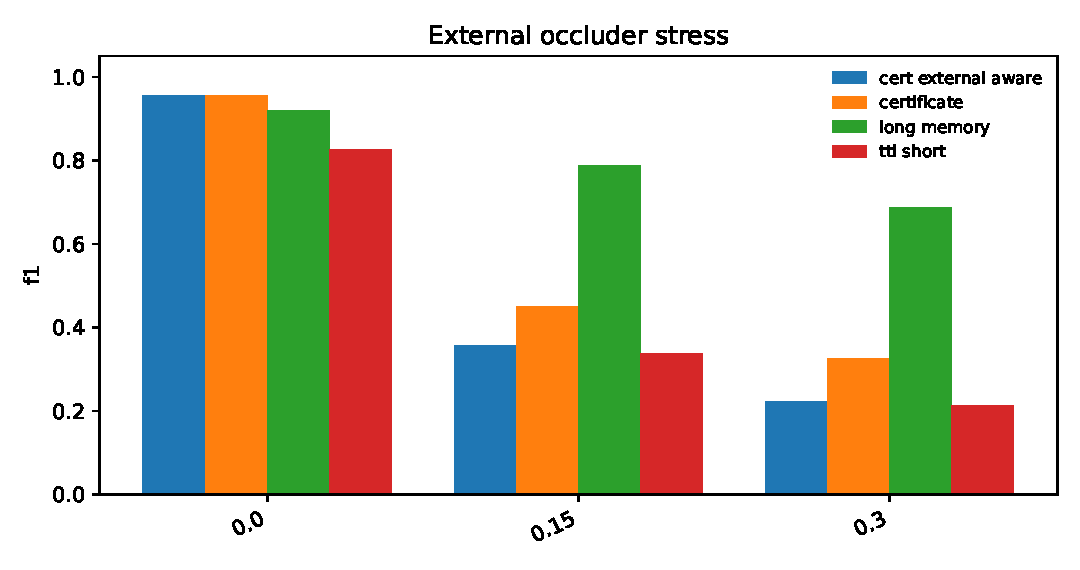
\includegraphics[width=0.82\linewidth]{../results/full_scale/figure_external_occluders.pdf}
\caption{Mixed-cause misses expose the limit of robot-only certificates.}
\label{fig:external}
\end{figure}

\subsection{Association And Re-Identification}

Family E removes the perfect-ID assumption. Table~\ref{tab:association} shows
that the certificate policy remains above short TTL even at high ambiguity and
30\% association swaps, but identity switches grow sharply. A real robot must
therefore combine certificates with association and re-identification; the
certificate alone is not an identity tracker.

\begin{table}[t]
\centering
\caption{Association stress. The certificate protects persistence semantics but
does not solve identity switches.}
\resizebox{\linewidth}{!}{\begin{tabular}{lllll}
\toprule
Swap & Policy & F1 & ID switches & Survival \\
\midrule
0.000 & certificate & 0.960 & 0.000 & 1.000 \\
0.000 & long\_memory & 0.930 & 0.000 & 1.000 \\
0.000 & oracle\_visibility & 0.975 & 0.000 & 1.000 \\
0.000 & ttl\_short & 0.821 & 0.000 & 0.956 \\
0.150 & certificate & 0.951 & 212.444 & 1.000 \\
0.150 & long\_memory & 0.931 & 212.444 & 0.949 \\
0.150 & oracle\_visibility & 0.968 & 123.222 & 1.000 \\
0.150 & ttl\_short & 0.797 & 212.444 & 0.664 \\
0.300 & certificate & 0.920 & 413.556 & 1.000 \\
0.300 & long\_memory & 0.916 & 413.556 & 0.905 \\
0.300 & oracle\_visibility & 0.962 & 237.111 & 1.000 \\
0.300 & ttl\_short & 0.769 & 413.556 & 0.410 \\
\bottomrule
\end{tabular}
}
\label{tab:association}
\end{table}

\begin{figure}[t]
\centering
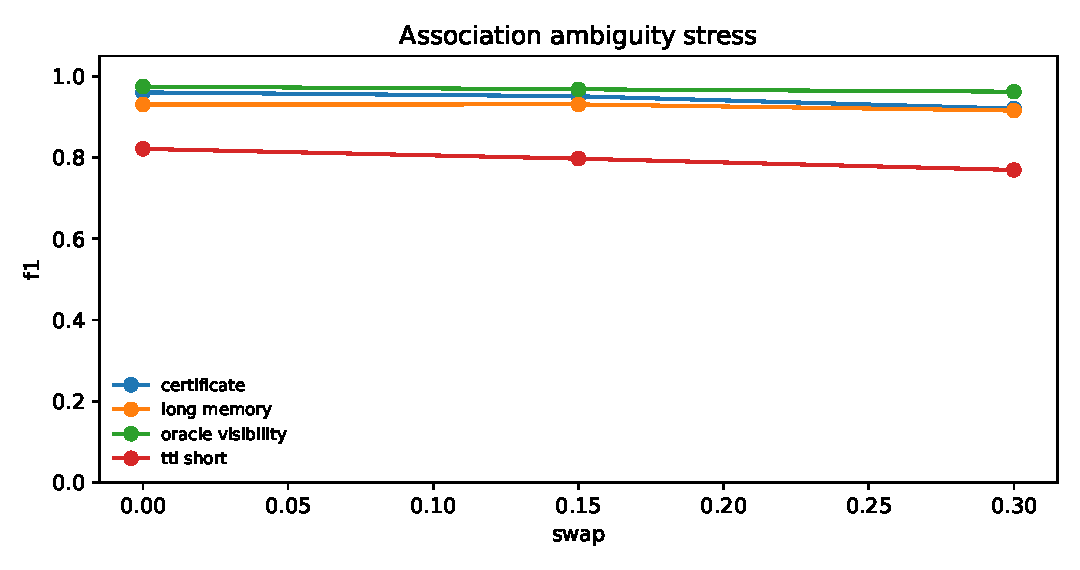
\includegraphics[width=0.82\linewidth]{../results/full_scale/figure_association.pdf}
\caption{Association ambiguity remains a deployment blocker.}
\label{fig:association}
\end{figure}

\subsection{Hidden Motion And Contact Displacement}

Family F tests objects that move while hidden. Table~\ref{tab:hidden} shows
that the certificate policy maintains strong presence F1, but reappearance
error increases under robot-contact displacement. Presence persistence is not
state accuracy. A robot that preserves a hidden object still needs a motion
model or contact model for where the object will be after occlusion.

\begin{table}[t]
\centering
\caption{Hidden-motion stress. Preserving presence does not guarantee accurate
hidden-state prediction.}
\resizebox{\linewidth}{!}{\begin{tabular}{lllll}
\toprule
Motion & Policy & F1 & Reappear err. & Stale \\
\midrule
drift & cert\_hazard & 0.962 & 0.314 & 0.150 \\
drift & certificate & 0.962 & 0.314 & 0.150 \\
drift & long\_memory & 0.927 & 0.314 & 0.554 \\
external & cert\_hazard & 0.969 & 0.291 & 0.197 \\
external & certificate & 0.969 & 0.291 & 0.197 \\
external & long\_memory & 0.943 & 0.291 & 0.517 \\
robot\_contact & cert\_hazard & 0.957 & 0.539 & 0.240 \\
robot\_contact & certificate & 0.957 & 0.539 & 0.240 \\
robot\_contact & long\_memory & 0.938 & 0.539 & 0.482 \\
static & cert\_hazard & 0.974 & 0.000 & 0.104 \\
static & certificate & 0.974 & 0.000 & 0.104 \\
static & long\_memory & 0.942 & 0.000 & 0.480 \\
\bottomrule
\end{tabular}
}
\label{tab:hidden}
\end{table}

\begin{figure}[t]
\centering
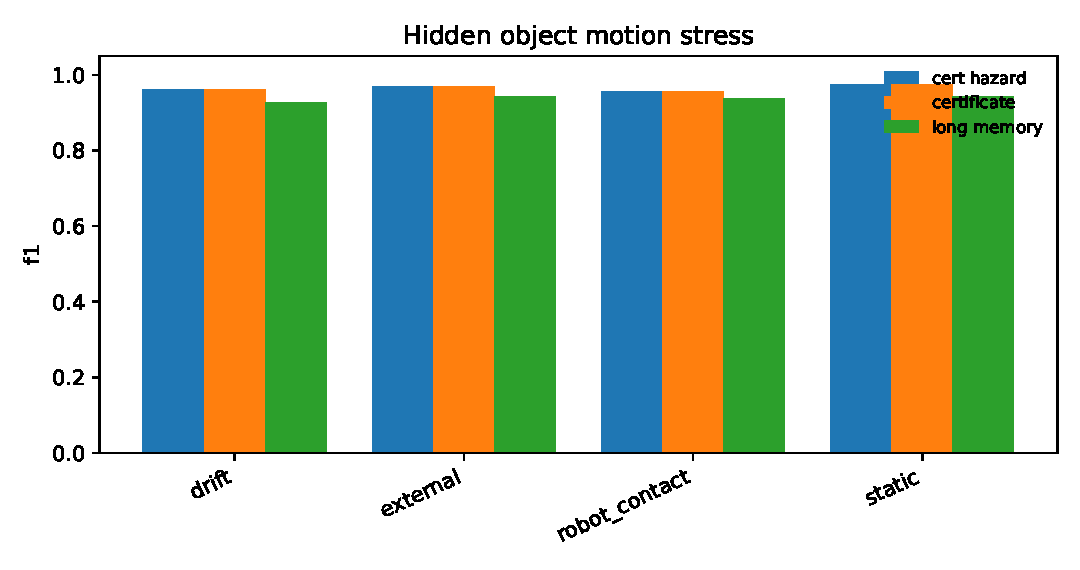
\includegraphics[width=0.82\linewidth]{../results/full_scale/figure_hidden_motion.pdf}
\caption{Hidden motion exposes the difference between object presence and
state accuracy after reappearance.}
\label{fig:hidden}
\end{figure}

\subsection{Stronger Persistence Baselines}

Family G compares stronger alternatives under mixed external occlusion. Long
memory obtains high F1 but with high stale clear-absence. Amodal proxy keeps
objects aggressively and therefore has stale clear-absence near 0.978. The
certificate and cert-hazard variants have lower F1 in this mixed-cause setting
but much lower stale clear-absence. This is the correct boundary: robot
self-occlusion certificates are not a universal memory replacement.

\begin{table}[t]
\centering
\caption{Stronger persistence baselines under mixed occlusion. Different
methods optimize different points on the persistence/staleness frontier.}
\resizebox{\linewidth}{!}{\begin{tabular}{lllll}
\toprule
Policy & F1 & Keep & Stale & Clear miss \\
\midrule
long\_memory & 0.899 & 0.790 & 0.488 & 0.001 \\
amodal\_proxy & 0.881 & 0.853 & 0.978 & 0.002 \\
kalman\_missing & 0.831 & 0.498 & 0.228 & 0.004 \\
hazard\_filter & 0.732 & 0.271 & 0.095 & 0.005 \\
cert\_hazard & 0.723 & 0.531 & 0.078 & 0.004 \\
certificate & 0.723 & 0.531 & 0.078 & 0.004 \\
ttl\_medium & 0.721 & 0.239 & 0.081 & 0.006 \\
ttl\_short & 0.580 & 0.080 & 0.034 & 0.004 \\
\bottomrule
\end{tabular}
}
\label{tab:baselines}
\end{table}

\begin{figure}[t]
\centering
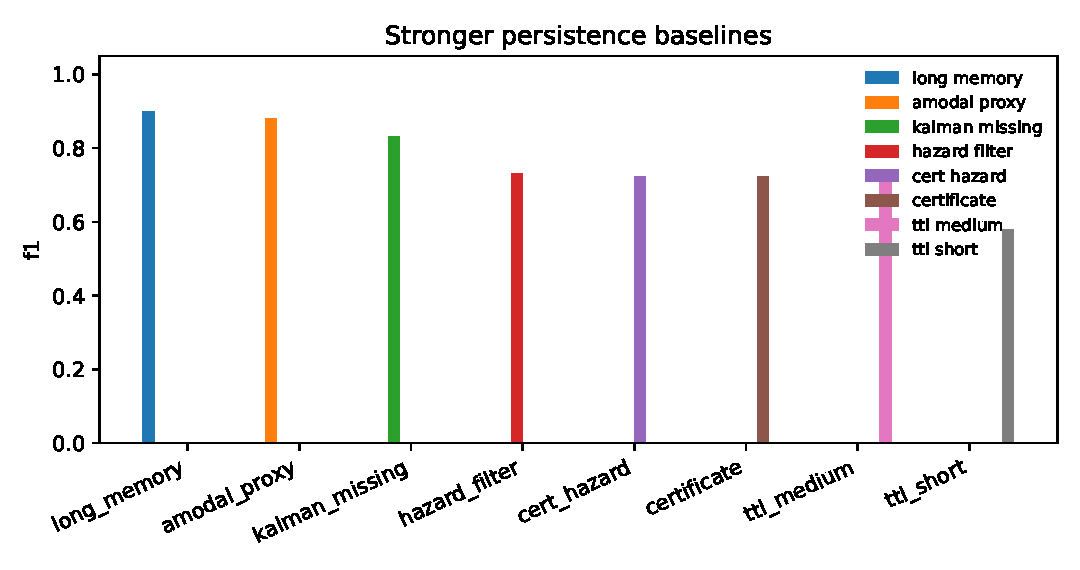
\includegraphics[width=0.82\linewidth]{../results/full_scale/figure_strong_baselines.pdf}
\caption{Long memory can improve F1 by preserving stale state; certificate
methods are designed to preserve specifically under robot-caused invisibility.}
\label{fig:baselines}
\end{figure}

\subsection{Ablations}

Family H isolates the semantics. No robot action and random geometry both
collapse because the certificate is no longer tied to the robot's actual
visibility. Underbroad certificates delete hidden objects; overbroad and
external-as-self variants preserve more but risk stale state. Oracle visibility
has perfect certificate precision/recall but still faces mixed-cause limits.

\begin{table}[t]
\centering
\caption{Ablations and negative controls. The visibility predicate must be tied
to robot action and must not be overbroad.}
\resizebox{\linewidth}{!}{\begin{tabular}{llllll}
\toprule
Policy & F1 & Keep & Stale & Cert prec. & Cert rec. \\
\midrule
external\_as\_self & 0.922 & 0.797 & 0.206 & 0.433 & 0.998 \\
no\_clear\_delete & 0.879 & 0.848 & 0.986 & 0.814 & 0.994 \\
overbroad\_certificate & 0.764 & 0.580 & 0.156 & 0.461 & 0.997 \\
certificate & 0.652 & 0.435 & 0.088 & 0.845 & 0.995 \\
oracle\_visibility & 0.645 & 0.428 & 0.026 & 1.000 & 1.000 \\
random\_geometry & 0.582 & 0.108 & 0.036 & 0.303 & 0.349 \\
underbroad\_certificate & 0.530 & 0.137 & 0.020 & 0.812 & 0.449 \\
no\_robot\_action & 0.514 & 0.061 & 0.017 & 0.000 & 0.000 \\
\bottomrule
\end{tabular}
}
\label{tab:ablation}
\end{table}

\begin{figure}[t]
\centering
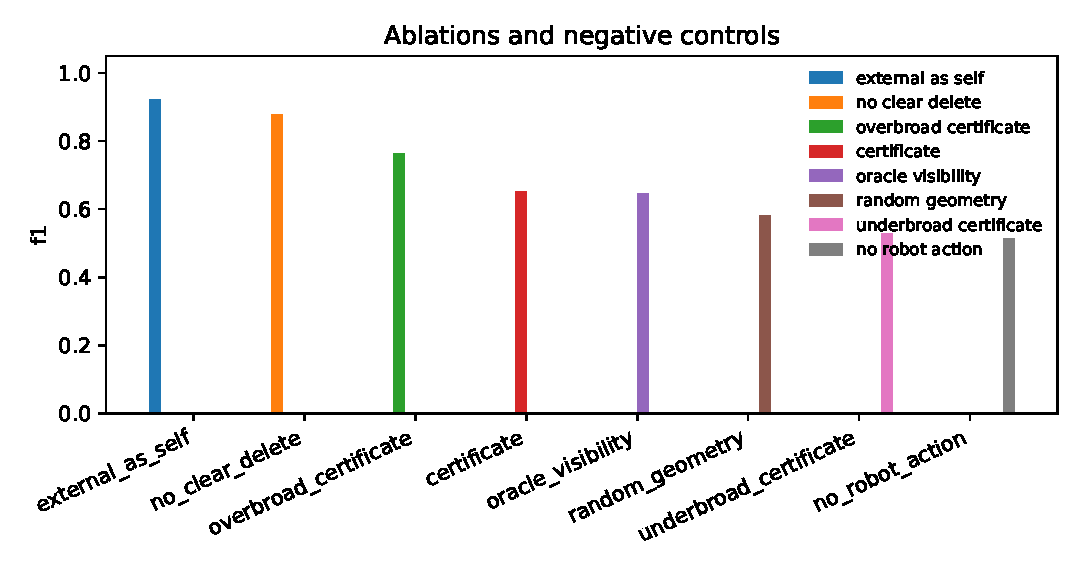
\includegraphics[width=0.82\linewidth]{../results/full_scale/figure_ablation.pdf}
\caption{Negative controls confirm that generic or random geometry is not
enough.}
\label{fig:ablation}
\end{figure}

\section{Discussion}

\paragraph{What the result supports.}
The suite supports the mechanism claim: missed detections should be interpreted
through robot-action visibility semantics. In self-occlusion regimes, the
certificate policy improves the persistence/staleness tradeoff relative to
short TTL and long memory.

\paragraph{What the result does not support.}
The suite does not prove real robot performance. It does not solve segmentation,
association, calibration, external occluder labeling, contact displacement, or
amodal shape inference. Several tables intentionally show cases where the
certificate is not the highest-F1 method because the setting includes mixed
occlusion causes that require additional models.

\paragraph{Design implication.}
The robot should expose the cause of a miss to the persistence layer. A miss in
clear view is absence evidence. A miss under robot-certified self-occlusion is
weak absence evidence. A miss under external occlusion is neither; it needs a
different uncertainty model.

\section{Limitations}

The evidence is synthetic. The simulator uses simplified angular visibility,
compact object states, and summary-level association stress. There is no real
camera, calibrated link mask, depth segmentation, robot-state latency log,
external occluder labeler, or contact-rich object displacement validation. The
strongest claim is therefore mechanism-level: robot action changes the semantics
of missed detections. A systems claim requires real robot sequences.

\section{Conclusion}

Robot self-occlusion turns object persistence from a generic memory problem into
an action-conditioned observability problem. Occlusion certificates are a small
mechanism, but they change the update rule: clear-view misses delete, while
robot-certified misses preserve. The v3 suite supports this mechanism and maps
its boundaries. Certificates must be calibrated, association-aware, and
separated from external occlusion before they can become a real robot
perception module.

\bibliography{references}
\bibliographystyle{iclr2026_conference}

\appendix
\renewcommand{\thesection}{\arabic{section}}

\section{Proof Details}

\subsection{Non-Identifiability With Miss Symbols}

The main proposition applies to any estimator that receives only a sequence of
miss symbols. The estimator may be Bayesian, deterministic, recurrent, or
learned. If its input is identical in two worlds, its update distribution is
identical. The robot visibility predicate provides an additional variable that
is not a function of detections alone.

\subsection{Certificate Soundness And Completeness}

Call a certificate sound if $C_t(\hat x_t)=1$ implies the robot actually blocks
the predicted object state. Soundness controls stale preservation. Call it
complete if every true robot self-occlusion is certified. Completeness controls
false deletion. A perfect certificate has both, but real geometry often trades
them. Inflation improves completeness and hurts soundness; shrinkage does the
opposite. Family B and Family C measure this tradeoff.

\subsection{False Positive Effect}

A false positive marks a clear-view miss as robot-caused unobservability. If the
object has been removed, the deletion counter is frozen and stale state
persists. This is why false positives primarily increase stale clear-absence.

\subsection{False Negative Effect}

A false negative marks true robot self-occlusion as clear view. If the object is
present but hidden, the deletion counter advances and the tracker can delete a
real object. This is why false negatives primarily lower keep-under-self-
occlusion and survival.

\section{Parameter Grids}

\subsection{Family A}
Family A uses widths 18, 42, and 60 degrees; speeds 0.5 and 1.0; object counts
8 and 16; detection probabilities 0.90 and 0.98; seven policies; three seeds
per cell; and three episodes per seed row. The main table reports the
42-degree slice averaged over the other axes.

\subsection{Family B}
Family B uses certificate noise values 0, 3, 6, 10, and 16 degrees; inflation
0, 2, and 6 degrees; robot-state latency 0, 1, 3, and 6 frames; and three seeds
per cell. The table reports latency 3.

\subsection{Family C}
Family C uses false-negative and false-positive rates 0, 0.25, 0.50, and 0.75,
with independent and bursty error modes.

\subsection{Family D}
Family D uses external occluder rates 0, 0.15, and 0.30; long external
occluder durations; labeled and unlabeled external causes; and short TTL, long
memory, certificate, and external-aware certificate policies.

\subsection{Family E}
Family E uses association swap rates 0, 0.15, and 0.30; low and high ambiguity;
and oracle visibility, certificate, short TTL, and long memory policies.

\subsection{Family F}
Family F uses static objects, passive drift, robot-contact displacement, and
external displacement, with correct and wrong hidden-motion models.

\subsection{Family G}
Family G compares short TTL, medium TTL, long memory, certificate, hazard
filter, Kalman-style missing-observation filter, amodal-memory proxy, and
certificate-hazard fallback under mixed occlusion.

\subsection{Family H}
Family H includes no robot action, random geometry, overbroad certificate,
underbroad certificate, no clear-view deletion, external-as-self, certificate,
and oracle visibility.

\section{Artifact Schema}

All v3 artifacts live under \path{results/full_scale/}. Each family writes a
seed CSV and a summary CSV. Figures are saved as PDF and PNG. Tables are saved
as LaTeX snippets and imported into the manuscript. The metadata file records
master seed 16016, family names, headline values, and seed-row counts.

\begin{table}[t]
\centering
\caption{Claim-to-evidence map generated by the v3 runner.}
\resizebox{\linewidth}{!}{\begin{tabular}{lll}
\toprule
Claim & Evidence & Result \\
\midrule
Self-occlusion is not a generic miss & Family A & cert F1 0.950 \\
Calibration has a precision/recall boundary & Family B & noise 6 F1 0.926 \\
False positives preserve stale objects & Family C & FP50 stale 0.293 \\
External occluders need separate semantics & Family D & external aware F1 0.357 \\
Association remains a deployment blocker & Family E & swap30 F1 0.920 \\
Ablations break the mechanism & Family H & random geom F1 0.582 \\
\bottomrule
\end{tabular}
}
\label{tab:claims}
\end{table}

\section{Reproducibility}

Run from the repository root:
\begin{verbatim}
python scripts\run_self_occlusion_experiment.py
python experiments\full_scale_occlusion_certificates.py
\end{verbatim}
Build from \path{paper/} with:
\begin{verbatim}
bibtex main
pdflatex -interaction=nonstopmode -halt-on-error main.tex
pdflatex -interaction=nonstopmode -halt-on-error main.tex
\end{verbatim}

\section{Calibration Checklist}

A real robot implementation should report the camera model, link masks,
robot-state timestamping, certificate inflation, calibration residuals, and the
certificate precision/recall against labeled self-occlusion. It should also
report latency stress, because stale joint states can turn a sound certificate
into a false positive or false negative.

\section{External Occluder Protocol}

External occlusion needs its own event. Treating every external occluder as
robot self-occlusion can preserve stale objects. Treating every external
occluder as clear view can delete real hidden objects. A deployed system should
separate robot self-occlusion, external occlusion, and clear-view absence. If it
cannot, it should propagate uncertainty rather than freezing or deleting
deterministically.

\section{Association Protocol}

The certificate tells the tracker whether the predicted object should be
visible. It does not solve which reappearing detection belongs to which object.
A real system needs association gates, appearance features, motion prediction,
and identity-switch metrics. Family E shows that association swaps grow under
ambiguity even when presence F1 remains strong.

\section{Hidden Motion Protocol}

Objects can move while hidden. A certificate can preserve presence, but state
prediction requires a motion model. Robot-contact displacement is especially
important because the robot body that hides the object may also move it. A
hardware follow-up should report reappearance localization error, not only
presence F1.

\section{Baseline Fairness}

Short TTL is the conservative deletion baseline. Long memory is the aggressive
persistence baseline. Hazard and Kalman-style filters represent probabilistic
miss handling. Amodal proxy represents a learned memory that tends to preserve
state. Oracle visibility gives the ceiling for robot self-occlusion semantics.
The certificate should be judged by the persistence/staleness tradeoff, not by
maximizing F1 in mixed-cause settings where long memory can win by preserving
stale objects.

\section{Detailed Simulator Semantics}

The simulator is intentionally compact, but the event semantics mirror the
failure that appears in manipulation. Each episode contains a set of object
slots with angular positions in a camera-centered field of view. A robot arm
sweeps through the field of view, producing time-varying self-occlusion
intervals. Objects may remain present for the whole episode or be removed after
a sampled time. A visible existing object is detected with a configurable
probability. A self-occluded object is missed because the robot blocks the view.
An externally occluded object is missed for a non-robot reason. A removed object
is absent and therefore cannot be detected.

The tracker does not receive the true cause of every miss. It receives
detections and, for certificate policies, a robot-geometry predicate computed
from the predicted object state and the robot arm state. This distinction is
important. A certificate can be true when the object is absent, because it is
computed from the predicted state. That is the stale-track failure mode. A
certificate can also be false when the object is truly self-occluded, because
calibration, latency, or under-inflated geometry can miss the blocked region.
That is the false-deletion failure mode.

The simulator also maintains a predicted angle for each track. In the static
case, this state remains correct under occlusion. In hidden-motion conditions,
the object can drift, be displaced by robot contact, or be displaced by an
external cause. The certificate can preserve the presence bit through these
intervals, but it cannot guarantee that the predicted state is still accurate.
This is why Family F reports reappearance error as well as F1. Persistent
presence and persistent pose are different goals.

External occlusion is simulated as a separate process. When external occluders
are unlabeled, the robot-only certificate cannot tell whether a miss under
external obstruction should preserve or delete. When external occluders are
labeled, the external-aware policy refuses to treat them as robot
self-occlusion. This reduces stale preservation but can lower F1 because the
system lacks a full external-occlusion memory model. This design is deliberate:
it prevents the paper from claiming that robot self-occlusion certificates solve
all missing observations.

\section{Metric Definitions}

\paragraph{Object-state F1.}
F1 is computed from frame-object presence decisions. A true positive is an
existing object whose track is present. A false negative is an existing object
whose track has been deleted. A false positive is an absent object whose track
remains present. A true negative is an absent object with no active track. This
metric rewards persistence but can hide the reason persistence occurs.

\paragraph{Keep-under-self-occlusion.}
This metric is the fraction of frames in which an object exists and is hidden by
the robot body for which the tracker keeps the track. It isolates the benefit
the certificate is designed to provide. Short TTL fails here because self-
occluded misses consume deletion budget.

\paragraph{Stale clear-absence.}
This metric is the fraction of frames in which an object is absent and not
self-occluded for which the tracker still keeps the track. It isolates the cost
of over-persistence. Long memory fails here because every miss is treated as
temporarily harmless.

\paragraph{External stale absence.}
This metric is the stale rate when an absent predicted state is externally
occluded. It is useful because external occlusion is neither clear-view absence
nor robot self-occlusion. A robot-only certificate should not silently absorb
this case.

\paragraph{Certificate precision and recall.}
Certificate precision measures how often a certificate corresponds to true
robot self-occlusion. Certificate recall measures how often true robot
self-occlusion is certified. Precision controls stale preservation; recall
controls false deletion. The calibration table reports both because F1 alone
does not reveal which side of the visibility tradeoff failed.

\paragraph{Occlusion survival.}
Survival measures whether a track that existed before a self-occlusion interval
is still present when the object reappears. This metric captures a common robot
failure: the object is still physically there, but the tracker deleted it while
the arm passed in front of the camera.

\paragraph{Reappearance error.}
Reappearance error measures state accuracy after hidden motion. A tracker can
have high presence F1 and still localize the object poorly after it reappears.
This is why hidden-motion experiments are not redundant with persistence
experiments.

\section{Calibration And Latency Guidance}

A certificate depends on robot geometry, camera calibration, robot state, and
the predicted object state. Each source can create a different failure. Camera
extrinsic error shifts the robot mask in image space. Link-shape error makes the
mask too thin or too wide. Timestamp latency evaluates the robot at a past
configuration. Prediction error asks whether the robot hides the wrong object
location. These errors combine nonlinearly: a certificate can be precise at one
arm speed and overbroad at another.

The practical response is to report a calibration surface, not a single
certificate setting. Family B uses geometry noise, inflation, and latency to
approximate this surface. Inflation is the easiest knob to understand. If the
robot expands its self-occlusion mask, recall improves because more true
self-occlusions are covered. Precision can drop because clear-view misses near
the mask edge are now treated as robot-caused. If the robot shrinks the mask,
precision can improve, but real self-occlusions become clear misses and tracks
are deleted.

Latency has a different signature. With a moving arm, a stale robot state shifts
the mask along the trajectory. The certificate can be correct before and after
an occlusion but wrong during the transition. This is especially dangerous for
fast manipulation, where the arm can enter and leave the camera ray between
perception frames. A hardware implementation should log camera timestamps,
joint-state timestamps, interpolation method, and maximum expected link-mask
motion per frame.

A real calibration checklist should therefore include: camera intrinsics and
extrinsics, link geometry source, robot mask rasterization method, timestamp
synchronization, inflation margin, validation images, labeled self-occlusion
precision, labeled self-occlusion recall, and stale-object rate in clear view.
The certificate is not a magical geometry oracle. It is a calibrated robot
self-visibility sensor.

\section{External Occlusion Taxonomy}

External occlusion is not one failure. It contains several cases with different
update semantics.

\paragraph{Temporary external occlusion.}
A person, tool, or object passes between the camera and the tracked object. The
object remains present, but the robot did not cause the miss. The correct update
may be to preserve with uncertainty, not to freeze deletion as if the robot
itself blocked the view.

\paragraph{External occlusion plus removal.}
An object is removed while another object blocks the view. Preserving the track
through this interval creates stale state. Robot self-occlusion certificates do
not solve this because the causal source is outside the robot's kinematic
model.

\paragraph{Robot and external overlap.}
The robot arm and an external occluder can overlap the same line of sight. A
robot certificate is true, but it is not the only cause of unobservability. The
system should mark this as mixed-cause unknown if external labels are available.

\paragraph{Unlabeled external occlusion.}
If the system cannot label external occlusion, it should avoid claiming a clean
self-occlusion certificate for all misses. A probability or uncertainty state is
safer than deterministic preservation.

Family D is intentionally hard on the certificate because it adds mixed causes.
The lower F1 of external-aware variants should not be read as a rejection of the
mechanism. It says that robot-only certificates need a companion model for
external occlusion. Long memory can score high in mixed-cause settings by
preserving many states, but the stale metrics reveal the cost.

\section{Association And Re-Identification Details}

Object persistence is not only a presence problem. When two visually similar
objects are near each other, a track can survive occlusion but attach to the
wrong reappearing detection. The certificate says whether the predicted object
should be visible; it does not say which detection is the same object. Family E
therefore injects association swaps and reports identity-switch counts.

The deployment implication is that certificates should be placed before
deletion, not after association. During self-occlusion, association evidence is
missing. The tracker should preserve the state and then use appearance,
geometry, and motion gates when detections return. If association confidence is
low at reappearance, the system should represent identity uncertainty rather
than immediately merging tracks.

The association stress also explains why object-state F1 can remain high while
identity quality degrades. Presence is a binary variable; identity is a matching
variable across time. A robot can know that an object still exists but not know
which of two reappearing cups is the original one. A systems paper must report
IDF1-like metrics, switch counts, and recovery after occlusion. This mechanism
paper reports a proxy switch count to mark that boundary.

\section{Hidden Motion And Contact Displacement}

Robot self-occlusion often occurs because the robot is near the object. That is
exactly when the robot may also move the object. A certificate preserves the
presence bit, but if the object is pushed while hidden, the predicted state can
be wrong. This is the difference between object permanence and state
prediction.

Family F separates static hidden objects, passive drift, robot-contact
displacement, and external displacement. The certificate retains high F1 because
presence remains true. Reappearance error grows under robot-contact
displacement, showing that a full system needs a contact-aware motion model.
The right architecture is not certificate versus physics. It is certificate for
miss semantics plus dynamics for hidden-state prediction.

This distinction matters in manipulation. A gripper can block a marker, push an
object, and then reveal it in a new pose. Deleting the object during the block
is wrong, but keeping the old pose unchanged is also wrong. The certificate
answers only the first part. A deployment system must update uncertainty or
state prediction during the certified interval.

\section{Real-Robot Dataset Design}

A real validation dataset should contain synchronized robot state, calibrated
camera frames, robot link masks, object detections, object IDs, and labels for
the cause of every miss. The labels should distinguish detected, clear-view
absence, robot self-occlusion, external occlusion, mixed occlusion, and unknown.
Without cause labels, the evaluation collapses back to generic missed
detections.

The dataset should include at least four regimes. First, static objects hidden
only by the robot body. This tests the core certificate. Second, removed
objects in clear view. This tests stale deletion. Third, external occluders
moving through the scene. This tests mixed-cause handling. Fourth, contact-rich
hidden motion, where the robot may move the object while hiding it. This tests
state prediction after persistence.

Metrics should be reported per regime. A single global F1 can hide the fact that
a method wins by preserving stale objects or by deleting too aggressively. The
minimum report should include F1, keep-under-self-occlusion, stale clear-
absence, external stale absence, survival, ID switches, and reappearance pose
error. The v3 synthetic suite is structured around these metrics so that a
hardware dataset can reuse the same evaluation vocabulary.

\section{Failure Taxonomy}

\paragraph{Underbroad certificate.}
The robot fails to certify true self-occlusion. The tracker consumes deletion
budget and loses real objects while the arm blocks the camera.

\paragraph{Overbroad certificate.}
The robot certifies clear-view absence as self-occlusion. The tracker preserves
removed objects and stale clear-absence rises.

\paragraph{Latency-shifted certificate.}
The robot mask is evaluated at the wrong time. This produces false positives on
one side of the moving arm and false negatives on the other.

\paragraph{External-cause confusion.}
The system treats external occlusion as robot self-occlusion or clear view.
Both can be wrong. Mixed-cause labels or uncertainty are needed.

\paragraph{Association survival without identity survival.}
The object remains present, but the track attaches to the wrong reappearing
detection. Presence F1 is not enough.

\paragraph{Presence survival without state survival.}
The track remains present, but hidden motion makes the state estimate wrong.
Reappearance error is required.

\section{Reporting Checklist}

A paper using robot self-occlusion certificates should report:
\begin{itemize}[leftmargin=*]
\item the robot geometry and camera calibration used to build certificates;
\item certificate precision and recall against labeled self-occlusion;
\item latency assumptions and timestamp synchronization;
\item deletion policy under clear-view misses;
\item behavior under false-positive and false-negative certificates;
\item external occluder handling;
\item association and identity-switch metrics;
\item hidden-motion or reappearance state error;
\item stale clear-absence in addition to F1;
\item ablations with no robot action, random geometry, overbroad certificates,
and underbroad certificates.
\end{itemize}

The current artifact satisfies this checklist synthetically. A systems paper
would need the same checklist on real robot data.

\section{Worked Scenarios}

\subsection{Arm Sweep Over A Present Object}

An object is detected on the table, and the robot arm moves between the camera
and the object for twelve frames. A short TTL tracker with patience three
receives twelve misses and deletes the object early in the occlusion. When the
arm moves away, the detector fires again, but the system must either create a
new track or re-identify the old one. The certificate tracker receives the same
misses, but the misses occur under robot-certified unobservability. Its
clear-miss counter does not advance, so the track survives. This is the intended
positive case.

\subsection{Object Removed In Clear View}

An object is detected, then a person removes it while the robot arm is not
blocking the camera. The detector emits misses in clear view. The certificate is
false, so the clear-miss counter advances and the track is deleted. Long memory
preserves the object for many frames and produces stale state. This is why the
paper reports stale clear-absence rather than only F1.

\subsection{Overbroad Robot Mask}

The robot's link mask is inflated too aggressively. A removed object near the
edge of the mask is labeled robot-occluded even though the camera would have
seen it if it were present. The certificate tracker freezes deletion and
preserves stale state. This is the false-positive boundary in Family C and the
overbroad ablation in Family H.

\subsection{Underbroad Robot Mask}

The mask is too narrow or the robot state is delayed. A real object is hidden by
the arm, but the certificate is false. The tracker treats the miss as clear
view and deletes a real object. This is the false-negative boundary. The
underbroad ablation has low stale rate but poor self-occlusion keep rate because
it behaves too much like short TTL.

\subsection{External Occluder}

A human hand blocks the object while the robot is elsewhere. A robot
self-occlusion certificate should not fire. The correct update is not obvious:
the object may still be present, but the robot did not cause the missing
evidence. A full system should represent external occlusion as a separate event
with its own uncertainty model. Family D shows that robot-only certificates are
not enough for this regime.

\section{Per-Family Interpretation}

\subsection{Family A Interpretation}

Family A is the cleanest test of the mechanism. It sweeps robot self-occlusion
width, arm speed, object count, and detection probability while keeping the
cause of misses mostly within the robot self-occlusion model. The certificate
policy improves over short TTL because it preserves objects during robot-caused
hidden intervals. It improves over long memory on stale clear-absence because
it still deletes when the object should have been visible. The oracle visibility
policy is a useful ceiling: the remaining gap to oracle reflects certificate
calibration, detection noise, and finite patience after clear misses.

\subsection{Family B Interpretation}

Family B is not only a stress test; it is a design tool. A robot developer can
read the calibration surface as a precision/recall tradeoff. If stale tracks
are the dangerous failure, the certificate should be biased toward precision:
smaller inflation, tighter masks, and possibly shorter preservation. If losing
hidden objects is the dangerous failure, the certificate should be biased toward
recall: larger inflation, slower deletion, or uncertainty-preserving updates.
There is no universally best setting because applications differ. A surgical
robot may prefer avoiding stale hallucinations; a warehouse manipulator may
prefer preserving bins through arm sweeps.

\subsection{Family C Interpretation}

Family C makes certificate errors causal. False negatives hurt the core benefit
because real self-occlusions are counted as clear misses. False positives hurt
the core safety property because clear-view absence is counted as robot
occlusion. The family is deliberately direct: it flips the certificate event
instead of hiding errors inside geometry. This makes the failure modes easy to
read. It also shows why certificate precision and recall should be reported
beside object F1.

\subsection{Family D Interpretation}

Family D explains why the paper avoids claiming generic object permanence.
External occlusion can make long memory look good by preserving objects through
many missing observations. But the same long memory preserves absent objects.
The external-aware policy refuses to call external occlusion robot
self-occlusion, which lowers stale rates but can lower F1 without a separate
external memory model. The right lesson is architectural: robot self-occlusion
is one event, not the only hidden-object event.

\subsection{Family E Interpretation}

Family E stresses identity. The certificate can keep a track alive through
robot occlusion, but if two objects are similar and near each other, the
reappearing detection can be assigned to the wrong identity. This is why a
real system must combine certificates with appearance and geometry association
gates. Presence persistence is necessary but insufficient for object-centric
robot memory.

\subsection{Family F Interpretation}

Family F stresses state accuracy. If the object moves while hidden, preserving
the track is not enough. The robot must also update uncertainty or motion
prediction. Robot-contact displacement is particularly important because the
same arm that causes occlusion may also move the object. The certificate should
therefore be paired with contact reasoning in manipulation.

\subsection{Family G Interpretation}

Family G is the strongest reminder that F1 is not the whole story. Long memory
and amodal proxy can obtain high F1 in mixed-cause settings by preserving many
objects, including stale ones. Certificate methods may rank lower on F1 while
having much lower stale clear-absence. A reviewer should therefore compare the
full metric vector, not a single scalar.

\subsection{Family H Interpretation}

Family H asks whether the geometry matters. No robot action and random geometry
perform poorly because the certificate is no longer tied to the actual cause of
missing evidence. Overbroad certificates preserve too much. Underbroad
certificates delete too much. Oracle visibility gives the clean self-occlusion
ceiling but does not solve external occlusion or association. These ablations
are the mechanism's fingerprint.

\section{Pseudocode}

The certificate-gated update can be implemented as the following local rule for
each track:
\begin{verbatim}
if detected(track):
    track.present = True
    track.clear_misses = 0
elif not track.ever_seen:
    pass
elif robot_cert(track.state, robot_state):
    track.clear_misses = track.clear_misses
else:
    track.clear_misses += 1
    if track.clear_misses > threshold:
        track.present = False
\end{verbatim}

A robust implementation should add uncertainty:
\begin{verbatim}
cause = classify_miss(robot_state, ext_occ, calib)
if cause == "robot_self_occlusion":
    preserve_with_robot_visibility_uncertainty(track)
elif cause == "clear_view":
    consume_deletion_budget(track)
elif cause == "external_or_unknown":
    propagate_unknown_occlusion(track)
\end{verbatim}
The second form is the one a real system should use. The first form is the
minimal mechanism isolated in the experiments.

\section{Real-Robot Acceptance Criteria}

A real-robot paper should satisfy several acceptance criteria before claiming
the mechanism works outside simulation.

\paragraph{Labeled miss causes.}
Every evaluation frame should label whether the object was detected, absent in
clear view, hidden by the robot, hidden by an external occluder, or unknown.
Without cause labels, the central semantic claim cannot be evaluated.

\paragraph{Calibrated robot masks.}
The system should project robot link geometry into the camera frame and compare
it against labeled robot occlusion. Precision and recall should be reported
across arm speeds and object depths.

\paragraph{Latency logs.}
Robot joint states and camera frames should be timestamped. The evaluation
should include a latency sensitivity analysis, because the certificate can be
wrong even with perfect geometry if it uses stale robot state.

\paragraph{Association metrics.}
Presence F1 should be accompanied by ID switches and re-identification success
after occlusion. Otherwise, a tracker can preserve the wrong identity and still
look good on presence.

\paragraph{State accuracy.}
If objects can move while hidden, the system should report reappearance pose
error or state uncertainty. A presence bit alone is not enough for manipulation.

\paragraph{Stale-object safety.}
The evaluation should report stale clear-absence and stale external-absence.
These are the metrics that prevent long memory from appearing better simply
because it refuses to delete.

\section{Why The Mechanism Is Not A Detector}

The certificate does not say that an object exists. It says that the robot
cannot use a miss as strong absence evidence because the robot blocked the
view. This distinction prevents a common overclaim. A detector or amodal model
estimates object state. A certificate estimates the observability of the
predicted state under robot geometry. The two are complementary.

This also explains why the certificate can be computed even when the object is
absent. The tracker has a predicted state from previous detections. The robot
can ask whether that predicted state would be visible. If the answer is no, a
miss is uninformative about absence. If the answer is yes, a miss is evidence
against persistence. The certificate changes evidence weighting; it does not
create positive evidence of existence.

\section{Why Generic Memory Is Not Enough}

Generic memory treats hidden state as a temporal smoothing problem. It can keep
objects alive through gaps, but it does not know which gaps were caused by the
robot and which gaps were clear-view absences. This is why long memory has high
stale clear-absence. A learned memory may reduce this if it implicitly learns
robot occlusion, but then the relevant question becomes whether the learned
state has access to calibrated robot geometry and whether it reports the same
precision/recall boundary. The certificate is an explicit version of that
information.

\section{Submission Boundary}

The submission-safe claim is: robot self-occlusion certificates improve the
semantics of missed detections for persistent object state in a controlled
mechanism suite. The unsafe claim is: the method solves object permanence for
real robots. The latter requires detector segmentation, calibrated link masks,
association, external occlusion labels, hidden-state dynamics, and hardware
logs. This paper supplies the mechanism and the evaluation vocabulary for that
future work.

\section{Systems Integration Notes}

A certificate-gated tracker should be integrated as an observability layer
between detection and deletion. It should not replace detection, association,
mapping, or dynamics. The detector proposes measurements. The association
module decides which track a measurement could update. The certificate layer
decides whether a missing measurement is informative. The state estimator then
updates presence and pose uncertainty. Keeping these roles separate prevents
the certificate from being used as positive evidence of existence.

In a real robot stack, the certificate can be computed from rendered link masks,
depth-buffer tests, ray casting against robot geometry, or conservative image
space masks. The implementation detail matters less than the validation:
certificate precision and recall must be measured against labeled robot
self-occlusion. A high-recall mask may be acceptable when stale tracks are not
dangerous. A high-precision mask may be required when stale state can cause
unsafe manipulation. The policy should be chosen from the task risk, not from a
single benchmark F1.

The persistence layer should also expose its event labels. Downstream planning
should know whether an object is detected, robot-occluded, externally occluded,
or stale/uncertain. A planner can then avoid relying on a stale pose, move the
arm to regain visibility, or request another camera view. If the perception
system hides these causes behind a single presence bit, it discards the very
information the robot action supplied.

\section{What Would Falsify The Mechanism}

Several outcomes would weaken the practical value of the mechanism. First, if a
real robot dataset showed that clear-view missed detections, robot self-occluded
misses, and external occluder misses all had the same optimal update rule, then
the event distinction would add little. This would not invalidate the
non-identifiability proposition, but it would make the mechanism unnecessary for
that domain.

Second, if calibrated robot masks had very low precision or recall across normal
manipulation motions, then certificates would be too unreliable to drive
deletion. In that case the correct conclusion would be that the robot needs
better calibration, multiple views, or learned visibility estimation before
certificate-gated persistence is safe.

Third, if association failures dominated every self-occlusion interval, then
presence preservation alone would not solve the user-visible problem. The
certificate would still be useful as observability information, but it would be
insufficient as a persistence system. A stronger paper would need identity-aware
tracking.

Fourth, if objects usually move substantially while hidden, preserving the last
state without a dynamics model could be harmful. This would push the method
toward uncertainty propagation rather than deterministic persistence. The
mechanism would remain useful for saying the miss was uninformative, but not for
saying the old pose is still accurate.

Finally, if an amodal or learned object-memory system already uses robot
geometry, external occluder labels, association uncertainty, and hidden-state
dynamics, then this paper's contribution becomes an explicit decomposition and
diagnostic vocabulary rather than a superior complete tracker. That is a
reasonable boundary: the paper's novelty is the update semantics, not ownership
of all persistent perception.

\section{Reviewer Self-Attacks}

\paragraph{This is just a hand-coded exception.}
The certificate is simple, but the point is the event semantics. Observation-only
misses are non-identifiable; robot action supplies additional information.

\paragraph{The simulator is synthetic.}
Correct. The paper is a mechanism submission. Hardware calibration, segmentation,
and association remain future work.

\paragraph{External occluders break the method.}
They break a robot-only certificate if treated as self-occlusion. Family D makes
this explicit and motivates mixed-cause event labels.

\paragraph{Long memory can have higher F1.}
Yes, when stale preservation is cheap in the metric. That is why stale
clear-absence is reported beside F1.

\paragraph{Amodal perception may solve hidden state better.}
Amodal perception can improve state prediction, but it still needs update
semantics for whether a miss is absence evidence. Certificates are complementary.

\section{Deployment Roadmap}

A real deployment should start with calibrated robot masks in camera space and
static tabletop objects. The next step is latency logging and inflation tuning.
Then association under clutter should be added, followed by external occluder
labels and hidden-motion prediction. Only after these stages should the method
be evaluated as a full persistent robot perception system.

\section{Active Re-Observation And Policy Choice}

The most useful deployment role for a certificate-gated tracker is not merely to
keep a Boolean object-present flag alive. It is to expose why the robot does not
know. A detected object has measurement support. A clear-view miss is evidence
against persistence. A certified self-occluded miss is a temporary loss of
observability caused by the robot's own action. An external-occluder miss is a
different latent event that may require waiting, changing viewpoint, or asking a
separate perception module to reason about the occluder. These labels are more
valuable than a single smoothed confidence score because they tell the robot
which action can reduce uncertainty.

This matters for active re-observation. When a track is self-occluded, the robot
can often choose a small corrective action: pause the arm sweep, retract a link,
move the wrist away from the camera ray, or request a second view before
executing a grasp. A generic memory tracker cannot distinguish this situation
from a detector dropout or true removal, so it has no principled reason to spend
motion budget on re-observation. A certificate tracker can trigger
re-observation exactly when the miss is uninformative because of robot geometry.
The policy does not need to trust the old pose blindly. It can mark the track as
present-but-unobserved, inflate pose uncertainty, and select an action whose
expected value is to make the predicted state visible again.

The evaluation in this paper intentionally does not optimize such a controller,
but the measured tradeoffs define the interface that a controller would need.
Family A says that a correct self-occlusion label recovers objects that a short
TTL tracker deletes. Family B says that calibration and latency determine whether
the label is precise enough to trust. Family C says that false negatives and
false positives cause different policy failures. A false-negative certificate
lets the deletion counter run during self-occlusion, so the robot may discard a
real object and fail to re-observe it. A false-positive certificate preserves a
track that should have been deleted, so the robot may waste time looking for an
object that has actually left. Family D then adds the main caution: if an
external occluder is folded into the self-occlusion class, the robot may choose
the wrong corrective action. Moving its own arm does not necessarily make a
human hand, tool, or unrelated object leave the camera ray.

The correct operating point is therefore task dependent. In a benign inventory
setting, stale tracks may be cheap and deleted present objects may be costly; a
high-recall certificate with conservative inflation can be acceptable. In
contact-rich manipulation, stale state can be dangerous because the robot might
plan through a pose that is no longer valid; a higher-precision certificate and
a faster clear-absence deletion rule may be preferred. In handover or
collaborative tasks, external occluders are common, so the robot should not treat
all hidden objects as self-occluded. The paper's tables report F1 because it is
a compact summary, but the deployment decision should compare stale
clear-absence, keep-under-self-occlusion, certificate precision, certificate
recall, and task loss separately.

This policy view also clarifies what ``final'' should mean for a future hardware
paper. A real robot result should not only report that object tracks survived an
arm sweep. It should report whether the robot knew why they survived, whether it
could recover visibility by acting, and whether that action reduced downstream
task loss. A minimal hardware protocol would label each miss by cause, log the
robot action chosen after the miss, record whether visibility was restored, and
compare against both short-memory and long-memory trackers under the same
motion budget. The expected result is not that certificates dominate every
metric. The expected result is that they make the uncertainty actionable: the
robot can choose to wait, re-observe, delete, or ask for a different view based
on the cause of missing evidence.

This distinction is the reason the negative results are part of the contribution.
The external-occluder family says the robot-only certificate should not be used
as a universal object permanence rule. The strong-baseline family says long
memory can win on aggregate F1 when stale tracks are not sufficiently penalized.
The ablation family says geometry-free persistence is not a substitute for
action-conditioned observability. Together these results turn the method from a
black-box persistence score into a policy contract: preserve objects during
robot-caused unobservability, delete them when absence is visible, expose
external and ambiguous causes instead of hiding them, and tune the certificate
from the task's asymmetric costs.

\section{Artifact-To-Claim Audit}

Family A supports the main self-occlusion semantics claim. Family B supports
the calibration boundary. Family C supports the false-positive/false-negative
boundary. Family D supports the external-occluder limitation. Family E supports
the association limitation. Family F supports the hidden-motion limitation.
Family G shows that stronger memory baselines optimize different tradeoffs.
Family H confirms that random or missing robot geometry is not enough. None of
these artifacts supports a claim of real-robot state of the art.

\section{Final Audit Paragraph}

The full-scale runner completed with stage \texttt{complete}, 1,124 seed-row
summaries, and zero plot failures. The manuscript imports generated v3 figures
and tables from \path{results/full_scale/}. The final claim is local and
mechanism-level: robot self-occlusion changes the semantics of missed detections
for persistent object state. The paper does not claim calibrated real robot
performance, solved association, external-occluder completeness, or contact-rich
hidden-state prediction.

\end{document}
